%\documentclass[12pt,draftclsnofoot,onecolumn]{IEEEtran}

\documentclass[10pt, twoside, jounal]{IEEEtran}
\usepackage{graphicx}
\usepackage{epstopdf}
\DeclareGraphicsExtensions{.pdf,.eps,.png,.jpg,.mps}
\usepackage[cmex10]{amsmath}
\usepackage{algorithm}
\linespread{1.00}
%\linespread{0.91}
\usepackage{algorithmicx}
\usepackage{algpseudocode}
\usepackage{bbm}
\usepackage[tight,footnotesize]{subfigure}
\usepackage{amssymb,amsmath}
\usepackage{epsfig}
\usepackage{times}
\usepackage{stfloats}
\usepackage{endnotes}

%\usepackage[utf,nonfrench,hangul,finemath]{kotex} % 한글 패키지

%\usepackage[nomarkers, nolists, tablesfirst]{endfloat}

\setlength{\parskip}{0em}     %문단제목사이 공백
%\setlength{\parindent}{1em}
\setlength{\textfloatsep}{5pt}   % 그림 캡션과 본문텍스트 사이 공백
\setlength{\abovedisplayskip}{0.1em}   %   수식 위쪽 공간 조절
\setlength{\belowdisplayskip}{0.1em}    %   수식 아래쪽 공간 조절
%%\setlength{\topskip}{0em}
%%\setlength{\columnsep}{0em}
%%\setlength{\topmargin}{0em}
%%\setlength{\abovecaptionskip}{0em}
%%\setlength{\belowcaptionskip}{0em}


\begin{document}

%1.\tiny
%2.\scriptsize
%3.\footnotesize
%4.\small
%5.\normalsize
%6.\large
%7.\Large
%8.\LARGE
%9.\huge
%10.\Huge

\title{
\LARGE
Deep RNN-based Traffic Analyzation Scheme for Detecting Target Applications \\
% Deep RNN-based Traffic Analyzation Scheme for Detecting Target Applications and Service Classes \\
% On-line Long Short-Term Memory(LSTM) based Traffic Analyzation Scheme (OL-TAS) with Intelligent Edge Computing (IEC) system
%Deep Long Short-Term Memory(LSTM) based Traffic Analyzation Scheme (DL-TAS) for Intelligent Edge Computing (IEC) system
%Deep Long short-term memory(LSTM) based Traffic Analyzation Scheme (LF-TAS) for Intelligent Edge Computing (IEC)
}

\author{Author 1, Author 2, Author 3, Author 4 and Author 5}

\maketitle

%%%%%%%%%%%%%%%%%%%%%%%%%%%%%%%%%%%%%%%%%%%%%%%%%%%%%%%%%%%%%%%%%%%%%%%%%%%%%%%%%%%%%%%%%%%%%%%%%%%%%%%%%%%%%%%%%%%%%%%%%%%%
% abstract
% 
%%%%%%%%%%%%%%%%%%%%%%%%%%%%%%%%%%%%%%%%%%%%%%%%%%%%%%%%%%%%%%%%%%%%%%%%%%%%%%%%%%%%%%%%%%%%%%%%%%%%%%%%%%%%%%%%%%%%%%%%%%%%
\begin{abstract}
This letter proposes a deep RNN-based traffic alayzation scheme for detecting target applications. The proposed scheme improves the classification performance in telecommunication networks with heavy traffic. In this work, we design a novel classification learning method where input features and output labels are two-dimensional image with traffic packet and target applications, respectively. 
Specifically, traffic packets are provided through universitat politecnica de catalunya barcelonatech as the training data\cite{Valentin2014}. 
Then, the proposed scheme provides a fast and exact traffic alayzation from the produced inferred function by analyzing the training data. We implement the proposed scheme using a commercial deep long short-term memory system. Simulation-based experiments show that the proposed scheme achieves almost xx\% accuracy performance with low complexity, requiring only xx ms elapsted time.
\end{abstract}

\begin{IEEEkeywords}
LSTM, Deep Learning, Network Traffic, Traffic Analyzation.
\end{IEEEkeywords}

\IEEEpeerreviewmaketitle

%%%%%%%%%%%%%%%%%%%%%%%%%%%%%%%%%%%%%%%%%%%%%%%%%%%%%%%%%%%%%%%%%%%%%%%%%%%%%%%%%%%%%%%%%%%%%%%%%%%%%%%%%%%%%%%%%%%%%%%%%%%%
% 1.introduction
% Related work 보완 필요
% CNN 기반 연구 등 기존 알고리즘의 장단점을 표현하고
% 본 논문의 아이디어를 직관적으로 설명이 필요하
%%%%%%%%%%%%%%%%%%%%%%%%%%%%%%%%%%%%%%%%%%%%%%%%%%%%%%%%%%%%%%%%%%%%%%%%%%%%%%%%%%%%%%%%%%%%%%%%%%%%%%%%%%%%%%%%%%%%%%%%%%%%

\section{Introduction}

\IEEEPARstart{V}{ARIOUS} types of applications and services are operatting in recent networks. It also provides easy access to the network from anywhere, including the smartphone, laptop, and desktop users. As the quality of demand increases, larger and more diverse traffic data is occurring.
Therefore, the scope of human data analysis and management is greatly expanding\cite{Park2009}. Therefore, it is necessary to establish a lightweight and automated network\cite{Risso2008}. In addition, the application of Deep Learning, which is gaining attention recently, is increasing.
Some of deep learning technologies include Multilayer Perceptron (MLP), CNN, and Recurrent Neural Network (RNN).
The MLP is a basic deep learning model consisting of approximately one or more hidden layers. CNN, which is a neural network that is comprised of three levels of local reception area, convolutional layer, and pooling layer, is a deep learning technique that is typically used in image analysis. RNN is a circular neural network suitable for processing random sequential data, and its characteristics are influenced by previous computational results. In this paper, RNN is used among deep learning techniques to classify network traffic based on flow.
The flow is a collection of the same traffic by 5-tuple, which in turn contains network packets. Therefore, RNN, which is suitable for training sequential data, is used for flow-based network traffic classification.
This requires a process of converting flow data collected on the network into a form that can be learned using RNN.
To this end, through the traffic data preprocessing process, the learning data generation step makes the raw traffic data divided by each application into traffic split and splited network traffic set easy to learn. The RNN learning will then categorize the flow.
Chapter 2 of this paper describes the system model, and Chapter 3 suggests deep RNN-based traffic analyzation sheme, and Chapter 4 conducts performance evaluation. Chapter 5 describes conclusions and future research plans.

%%%%%%%%%%%%%%%%%%%%%%%%%%%%%%%%%%%%%%%%%%%%%%%%%%%%%%%%%%%%%%%%%%%%%%%%%%%%%%%%%%%%%%%%%%%%%%%%%%%%%%%%%%%%%%%%%%%%%%%%%%%%
% 2. system_model
% 제안하는 스킴에 배경이 되는 시스템 모델 표현 필요 (추후 고려)
% IEC에 대한 시스템 모델 및 분류 예시를 나열한다
% 혹은 target application 및 service class 분류 
%%%%%%%%%%%%%%%%%%%%%%%%%%%%%%%%%%%%%%%%%%%%%%%%%%%%%%%%%%%%%%%%%%%%%%%%%%%%%%%%%%%%%%%%%%%%%%%%%%%%%%%%%%%%%%%%%%%%%%%%%%%%
\section{System Model}
{\it We need to express a system model that is behind the proposed scheme.}
%IEC에 대한 시스템 모델 및 분류 예시를 나열한다
%혹은 target application 및 service class 분류

%%%%%%%%%%%%%%%%%%%%%%%%%%%%%%%%%%%%%%%%%%%%%%%%%%%%%%%%%%%%%%%%%%%%%%%%%%%%%%%%%%%%%%%%%%%%%%%%%%%%%%%%%%%%%%%%%%%%%%%%%%%%
% 3.1 Preprocessing for Proposed Scheme
% 데이터 전처리 과정을 설명함 
%%%%%%%%%%%%%%%%%%%%%%%%%%%%%%%%%%%%%%%%%%%%%%%%%%%%%%%%%%%%%%%%%%%%%%%%%%%%%%%%%%%%%%%%%%%%%%%%%%%%%%%%%%%%%%%%%%%%%%%%%%%%

\section{Proposed deep RNN-based traffic analyzation sheme (DR-TAS)}
This chapter describes traffic data preprocessing and deep RNN model for Proposed deep RNN-based traffic analyzation scheme.

\subsection{traffic data preprocessing}
The traffic data used to perform traffic classifications is a preprocessing packet capture (PCAP) files supplied by universitat politecnica de catalunya barcelonatech (UPC) \cite{Valentin2014} suitable for RNN learning.
PCAP is a file that captures network packets and stores them in the form of PCAP files using programs such as Wireshark and TCPdump.
PCAP provided for flow-based network traffic classification using RNN suggested in this letter need to be pre-processed into data sets classifiable in RNN traffic anlyzation. This requires a data pre-processing process to filter and shorten the PCAP files.
The original PCAP file is approximately 59GB in size and has 769507 flows.
In the packet$\_$default.info file provided with the PCAP file, there is labeling for the traffic data.
Labeling is divided into classes, such as the application type, protocol, and application name for the corresponding traffic flow.
The labeling file gave us the correct label for ground truth in the flow-based traffic classification with RNN suggested in this letter.

For the data pre-processing process, eight types of applications were selected based on the number of flows. The top eight label names were Remote Desktop Protocol (RDP), Skype, SSH, Bittorrent, HTTP-face-Govert, HTTP-Doki, HTutube, and only the corresponding label selection flow.
Only the payload of the application layer was filtered out of the selected flow internal packet, and the extracted payload data was placed  and eight application layer Payload data files were generated. And for HTTP-facebook-Google, HTTP-Web, HTTP-Doki, HTTP-Youtube, we finally combined the label with the label Web to create a total of five data sets.
Through the integration process, the application layer Payload data files of RDP, Skype, SSH, Bittorrent, and Web were completed.
The data file has header information for each flow, and the payload separated by a $\#$ delimiter for each packet.
That is, each file is a collection of flows with the same label, with packets having only a payload and the payload being separated by a packet. The payload is also a string, with a size of four bits per one character. Figure 1 shows statistical information on the finished application layer Payload data file.

\begin{table}
\caption{statistical information of each application}
\setlength{\tabcolsep}{3pt}
\begin{tabular}{|p{65pt}|p{31pt}|p{31pt}|p{31pt}|p{31pt}|p{31pt}|}
\hline
 & rdp & skype & ssh & bittorrent & http-web \\ 
\hline
\hline
Total number of filtered flows & 153,349 & 2,041 & 38,831 & 96,222 & 21,715 \\ 
\hline
Total number of packets(K) & 6,876K & 3,015K & 173,911K & 207,306K & 47,136K \\ 
\hline
Average number of packets in a flow & 44 & 1,477 & 461 & 2,154 & 2,483 \\ 
\hline
Total packet size (GB) & 131.3 & 12.0 & 321.7 & 2,170 & 698.4 \\ 
\hline
Average packet size over all flows (KB) & 20.0 & 4.2 & 18.8 & 11.3 & 15.9 \\ 
\hline
Min packet size over all flows (B) & 8.0 & 8.0 & 8.0 & 8.0 & 8.0 \\ 
\hline
Max packet size over all flows (MB) & 5.5 & 0.3 & 6.6 & 0.8 & 40.0 \\ 
\hline
\end{tabular}
\label{tab1}
\end{table}

This step describes the process of converting LSTM into learning data using the application layer payload data generated in the previous step.
A data set for learning will have flight data with 8,750 flows, 1,250 validation data, and 2,500 test data. Each label data equal to the number of each transaction, validation, test data set.
Each application flow in the application layer payload data file goes through a conversion process into data for LSTM learning.
The conversion job removes the head information that indicates the flow id, start time, and end time of each flow, and imports the data portion of the application layer only the payload in the flow unit and creates a data set. The LSTM models should have the same number of data input at a time to perform the learning in flow units. That is, a flow should have the same size packets. For this purpose, the user can specify as many packets per flow as P. In addition, one packet in the flow has a user-designed size, which can be set by the user to N, and it has a one-dimensional array size. The pixels of a packet's pixel have a $2^n$ bit size and a character-type value replaced by a floating point value.
That is, the data in one flow will be the same size as the equation (1).
\begin{equation}
{\rm N_{flow}} = {\rm N \quad x \quad 2^n \quad  x \quad P} 
\end{equation}

Fig.\ref{fig1} shows the payload of a packet in one of the completed flows in an two-dimentional image, a element of four bits in size, and a value between zero and fifteen floating point. In addition, due to the nature of the LSTM network structure, all flows should have the same number of packets.Because the length of sequence is set in advance, the number of packets per flow should be the same by that length. However, since not all Applicatoin flows can have the same number of packets, if the number of packets per flow is smaller than the N set, then the packet is generated by zero.
Train, Validation and Test Label have labels for a total of five applications, which can be expressed as one-hot vectors of five lengths. A one-hot vector label having a value of only one element, can be defined as a label on which an index of one points to an application name. Table 2 shows the structure represented by the Train, Validation, and Test labels as on-hot vectors.

\begin{figure}[!t]
\centering
\setlength{\abovecaptionskip}{0pt}
\setlength{\belowcaptionskip}{0pt}
{
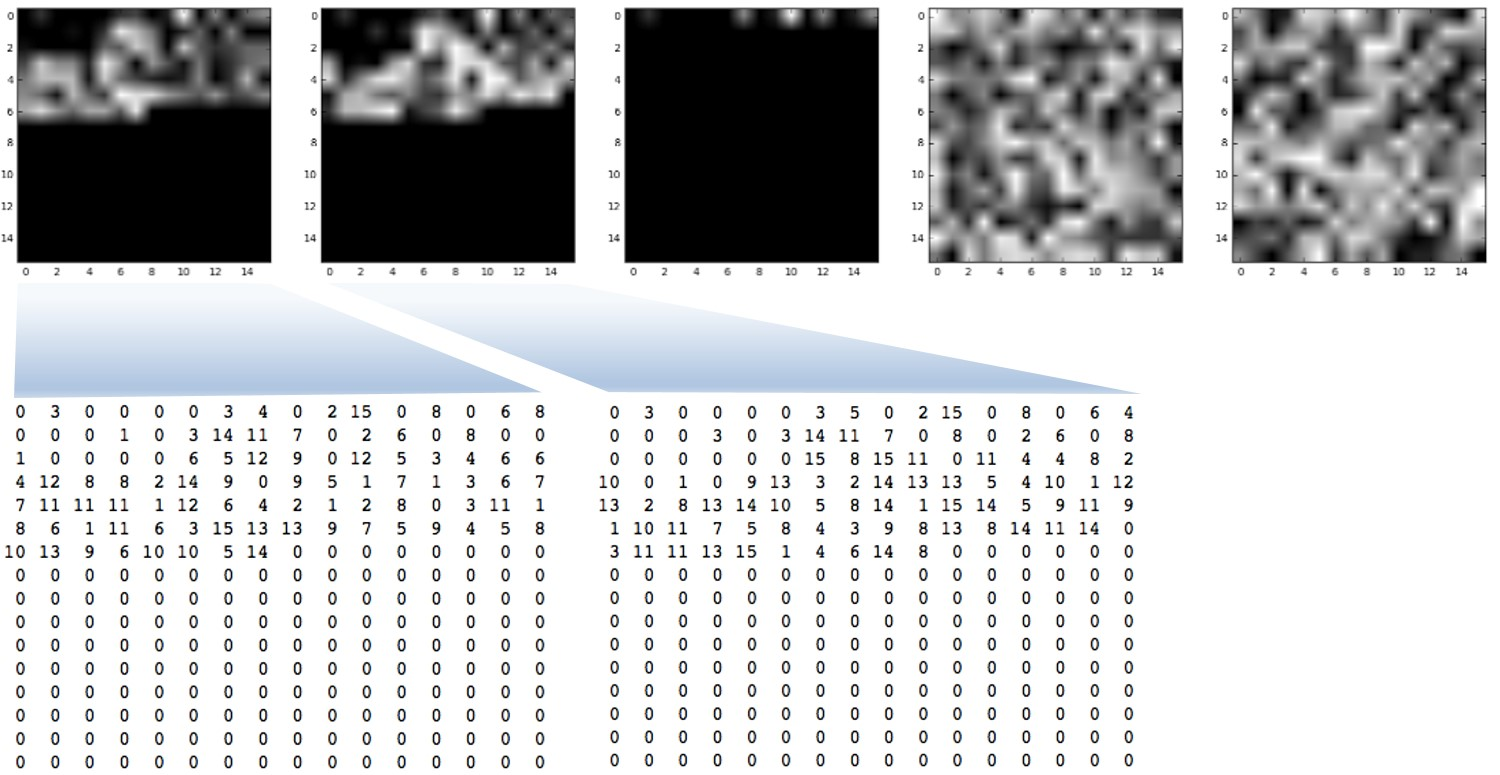
\includegraphics[width=3.6in, height=2.0in]{fig1.jpg}
\caption{Input features of flow packet}
\label{fig1}
}
\end{figure}
\begin{table}
\caption{output labels of application one-hot vector}
\setlength{\tabcolsep}{3pt}
\begin{tabular}{|p{55pt}|p{33pt}|p{33pt}|p{33pt}|p{33pt}|p{33pt}|}
\hline
 Application & RDP & Skype & SSH & Bittorrent & Web \\ 
\hline
\hline
label & [1,0,0,0,0] & [0,1,0,0,0] & [0,0,1,0,0] & [0,0,0,1,0] & [0,0,0,0,1] \\ 
\hline
\end{tabular}
\label{tab2}
\end{table}

%%%%%%%%%%%%%%%%%%%%%%%%%%%%%%%%%%%%%%%%%%%%%%%%%%%%%%%%%%%%%%%%%%%%%%%%%%%%%%%%%%%%%%%%%%%%%%%%%%%%%%%%%%%%%%%%%%%%%%%%%%%%
% 3.2 proposed RNN model
% LSTM 모델 구조 설명
%%%%%%%%%%%%%%%%%%%%%%%%%%%%%%%%%%%%%%%%%%%%%%%%%%%%%%%%%%%%%%%%%%%%%%%%%%%%%%%%%%%%%%%%%%%%%%%%%%%%%%%%%%%%%%%%%%%%%%%%%%%%
\subsection{Proposed deep RNN model}
This subsection describes the LSTM models that will be used for flow based network traffic classification using the proposed LSTM. LSTM shows great performance for various natural language processing (NLP) issues, especially LSTM is able to learn sequential data over CNN, which is used more by Deep Learning.
Therefore, we believe that the network traffic classification through LSTM will be accurate in analyzing the flow that contains sequential information of packets.
Fig.\ref{fig2} shows the learning structure of the Proposed deep RNN-based traffic analyzation sheme used to classify traffic, and the learning model consists of a single layer. The time step for learning LSTM is to preset the number of packets throughout the flow to be learned. Time steps represent the number of inputs a flow enters sequentially from a single layer to an LSTM. Therefore, the form of learning data sets is represented in the train data set (number of flows, number of packets per flow, and payload size per packet), and the label data (number of flows, number of labels).
The data sets of tests and validation are also inputted in the same form and learned through LSTM.
The problem with the existing vanilla RNN is that of long-term dependency if the length of sequence is longer. Thus, this network architecture utilizes LSTM, a solution to long-term dependency problems.

\begin{figure}[!t]
\centering
\setlength{\abovecaptionskip}{0pt}
\setlength{\belowcaptionskip}{0pt}
{
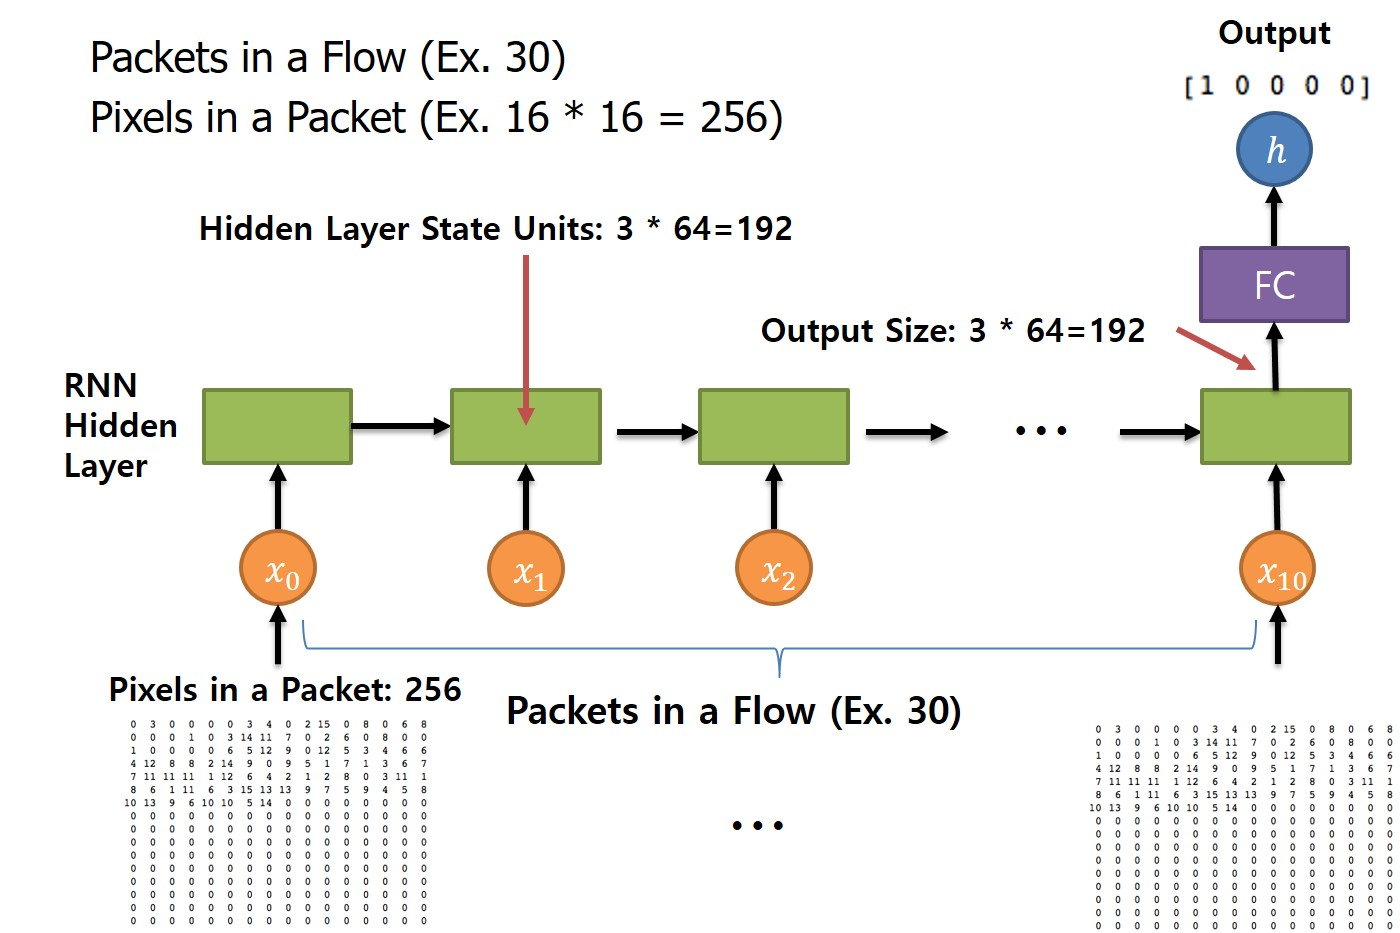
\includegraphics[width=3.6in, height=2.0in]{fig2.jpg}
\caption{Proposed deep RNN-based traffic analyzation sheme}
\label{fig2}
}
\end{figure}

%%%%%%%%%%%%%%%%%%%%%%%%%%%%%%%%%%%%%%%%%%%%%%%%%%%%%%%%%%%%%%%%%%%%%%%%%%%%%%%%%%%%%%%%%%%%%%%%%%%%%%%%%%%%%%%%%%%%%%%%%%%%
% 4.simulation_result
% 그래프 보완 필요
% 1) LSTM 자체 정확도 그래프
%    x축은 플로우당 패킷 개수, y축은 정확도, 
%    legend는 패킷당 페이로드 데이터수 (DR-TAS(40), DR-TAS(80), DR-TAS(160))
% 2) LSTM 의 각 application별 혹은 각 service class 별 정확도
%    막대 그래프 형태로, 
%    x축은 각 application별(혹은 각 service class별), y축은 정확도  
% 3) CNN vs LSTM 정확도 그래프
%    x축은 2,3,4,5 classifier, y축은 정확도
%    legend는 DC-TAS, DR-TAS
% 4) CNN vs LSTM elapsed time 그래프
%    x축은 2,3,4,5 classifier, y축은 inference elapsed time
%    legend는 DC-TAS, DR-TAS
% 5) 전체 프로세싱 time 
%    클라우드(모든 기능) vs. 에지(전처리 기능)+클라우드(ML 기능) 
%    vs 에지 (모든 기능) 비교 - 전체 프로세싱 시간 
%%%%%%%%%%%%%%%%%%%%%%%%%%%%%%%%%%%%%%%%%%%%%%%%%%%%%%%%%%%%%%%%%%%%%%%%%%%%%%%%%%%%%%%%%%%%%%%%%%%%%%%%%%%%%%%%%%%%%%%%%%%%

\section{Performance evaluation}
We compare DR-TAS to deep CNN-based traffic analyzation sheme (DC-TAS).
%본 장에서는 2장과 3장의 트래픽 데이터 처리 및 학습 데이터 생성 작업을 거친 데이터 세트를 LSTM 모델에 Feeding 하여 훈련시켰다. 플로우 단위의 데이터는 플로우 당 패킷의 개수에 따라 얼마만큼의 학습을 할지 결정할 수 있다. 또한 LSTM 훈련 시 한 셀에 들어가는 Input 데이터의 크기는 한 플로우의 한 패킷의 페이로드 사이즈와 동일하기 때문에 이 또한 플로우 기반의 분류에 영향을 줄 수 있다. 따라서, 본 논문에서 제안하는 플로우 기반의 네트워크 트래픽 분류를 위하여 플로우당 패킷의 개수와 플오우내 한 패킷의 페이로드 사이즈를 다르게 하여 실험 평가를 진행하였다.
%실험은 Ubuntu 14.04 LTS 환경에서 실험을 진행 하였고, RAM 32GB, NVIDIA GTX 1080Ti를 사용하였다. 또한, Tensorflow 환경에서 Python을 이용하여 트래픽 분류를 위한 RNN 학습을 수행하였다.
%실험 평가를 진행하기 위하여 한 플로우당 패킷의 개수를가 10, 30, 60, 100개로 하였으며, 한 패킷 당 페이로드 사이즈를 40, 80, 160으로 설정하였다. 각 Label은 그림4의 내용을 토대로 Label 데이터를 생성하였으며, 각 플로우 갯수는 Train, Validation, Test 별로 각각 8750개, 1250개, 2500개로 설정하였다. LSTM 네트워크의 배치 사이즈는 1000이며, LSTM의 Sequence Length는 플로우당 패킷의 개수와 동일하며, Hidden Size는 한 패킷 당 페이로드 사이즈와 동일하며, Hidden Size는 한 패킷 당 페이로드 사이즈와 동일하다. 최종 Output의 모양은 (플로우 개수, 5)의 형태로 출력된다. 
%그림7은 플로우당 패킷의 개수와 패킷의 페이로드 사이즈에 따른 Test Accuracy 결과를 나타낸다. 위 그림7에서 보이는 바와 같이 플로우 당 패킷의 개수가 증가함에 따라 전체적인 정확도도 올라가는 것을 볼 수 있다. 또한, 한 패킷의 페이로드 사이즈가 커지메 따라 정확도도 올라가는 것을 확인 할 수 있다. 따라서, 본 논문에서 제안하는 LSTM을 이용한 플로우 기반의 네트워크 트래픽 분류는 거의 99$\%$ 이상의 분류를 할 수 있으며, 데이터 사이즈가 커짐에 따라 그 정확도가 더 증가하는 것을 확인하였다.

\begin{figure}[!t]
\centering
\setlength{\abovecaptionskip}{0pt}
\setlength{\belowcaptionskip}{0pt}
{
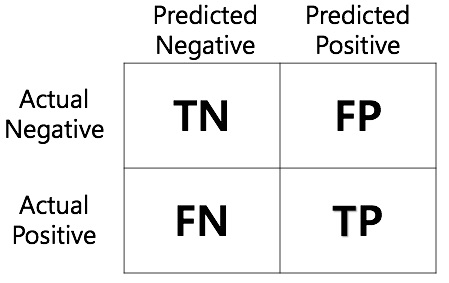
\includegraphics[width=3.6in, height=2.0in]{fig3.jpg}
\caption{Accuracy of deep RNN-based traffic analyzation scheme}
\label{fig3}
}
\end{figure}
\begin{figure}[!t]
\centering
\setlength{\abovecaptionskip}{0pt}
\setlength{\belowcaptionskip}{0pt}
{
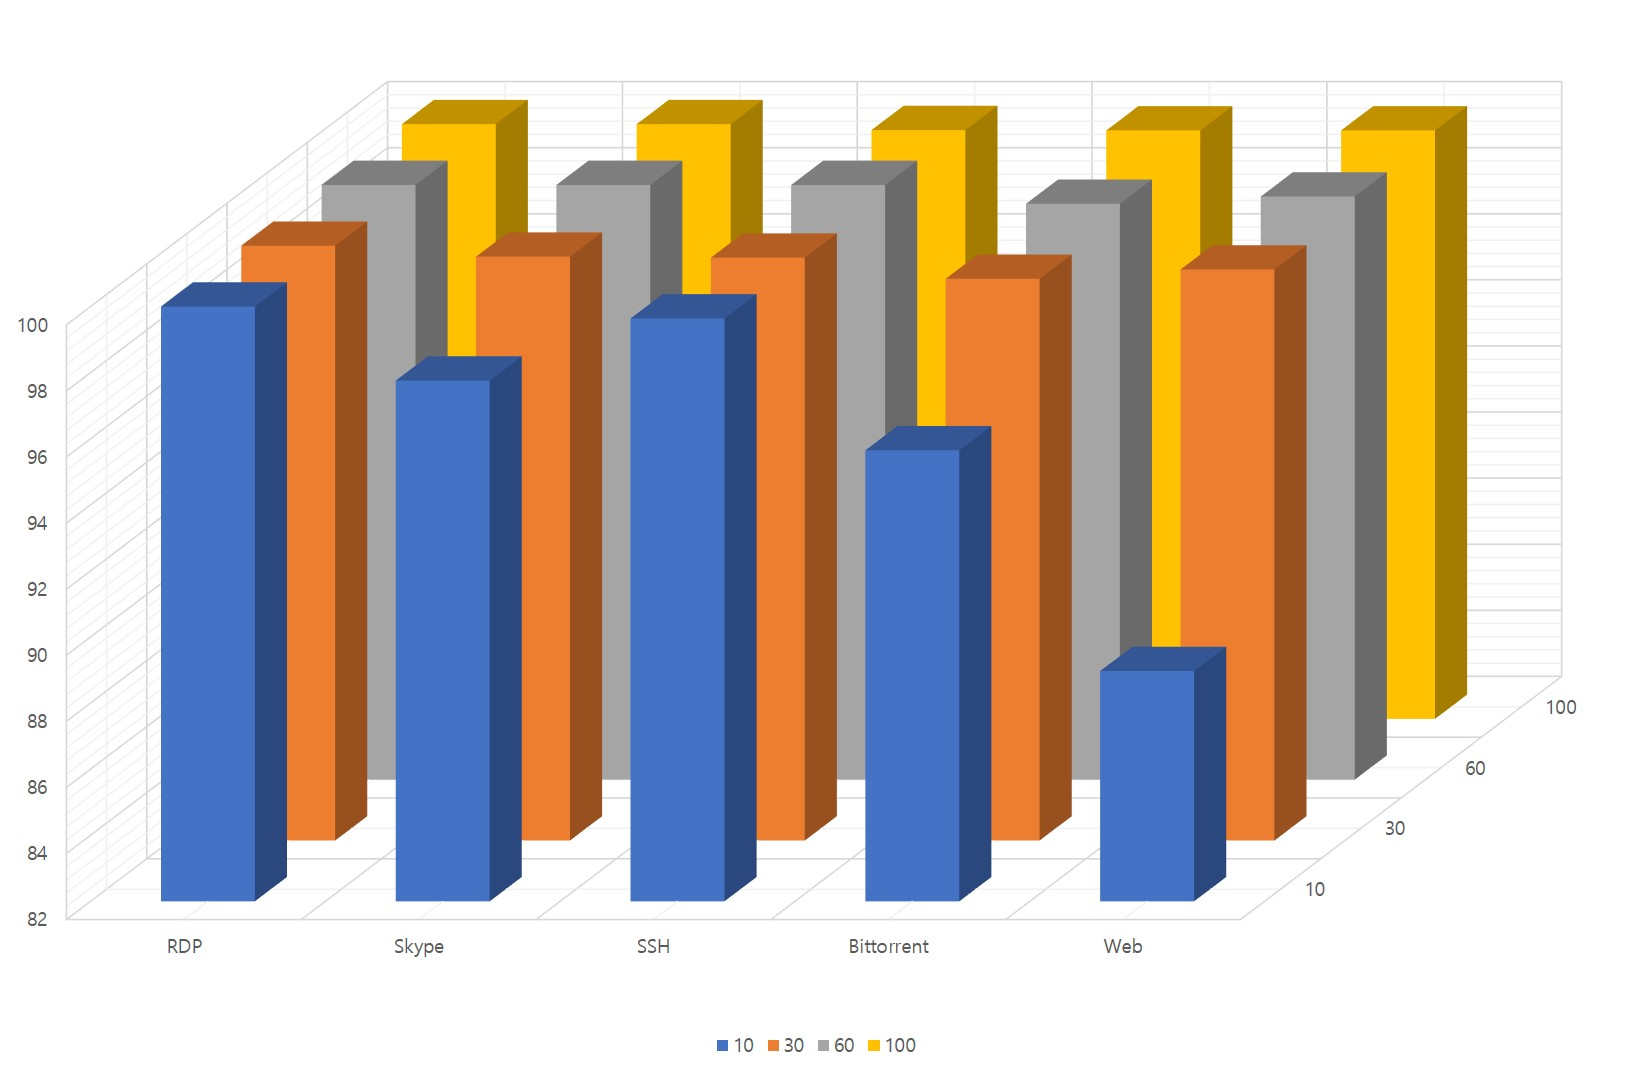
\includegraphics[width=3.6in, height=2.0in]{fig4.jpg}
\caption{Accuracy of DR-TAS for each target application}
\label{fig4}
}
\end{figure}

\begin{figure}[!t]
\centering
\setlength{\abovecaptionskip}{0pt}
\setlength{\belowcaptionskip}{0pt}
{
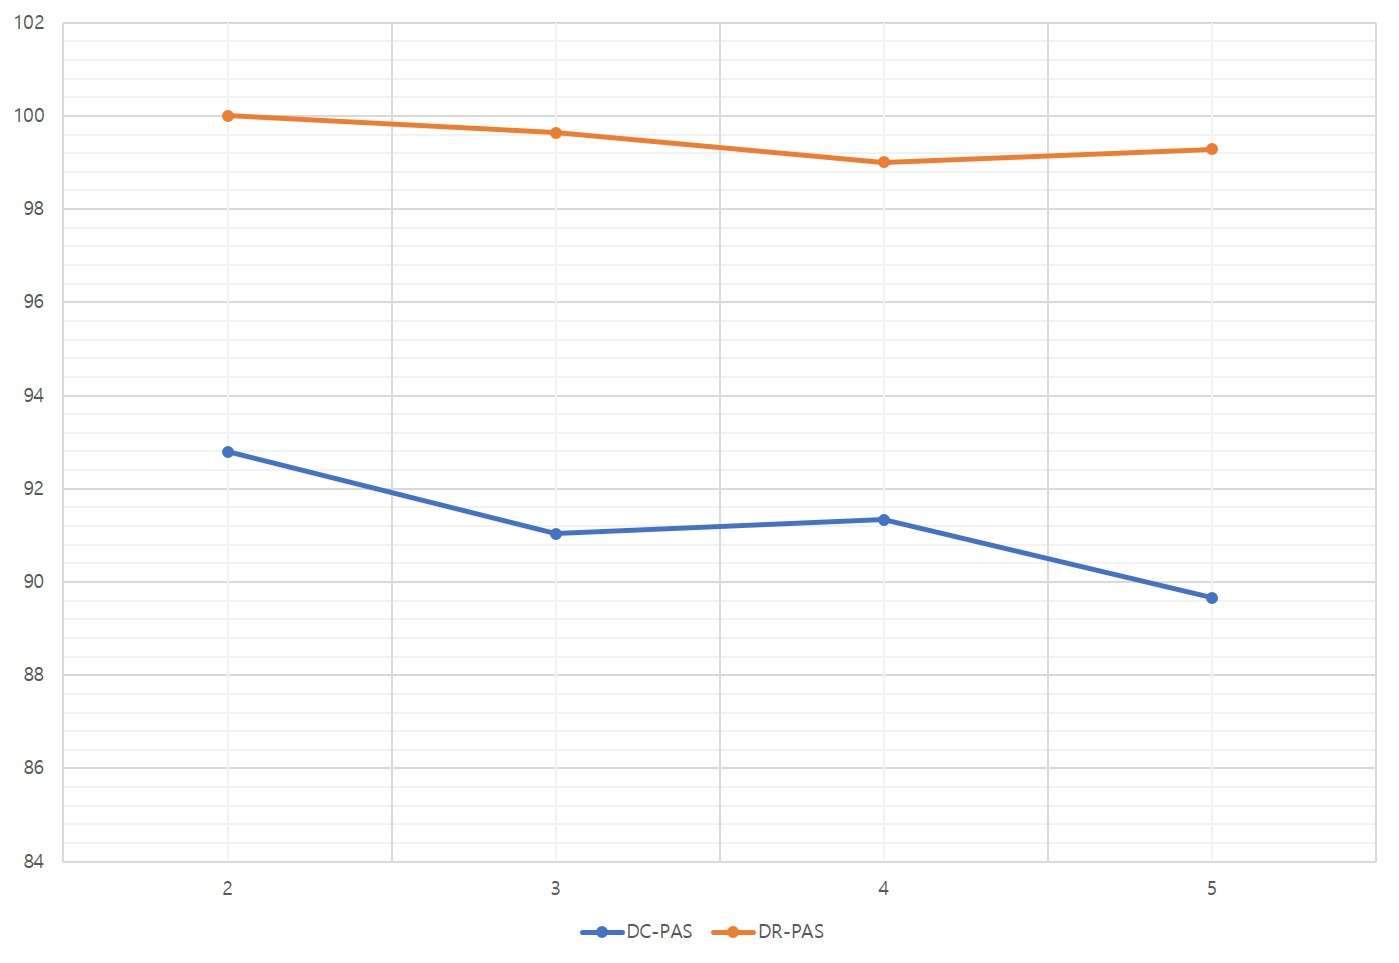
\includegraphics[width=3.6in, height=2.0in]{fig5.jpg}
\caption{Comparison on accuray of DR-TAS vs. DC-TAS }
\label{fig5}
}
\end{figure}

\begin{figure}[!t]
\centering
\setlength{\abovecaptionskip}{0pt}
\setlength{\belowcaptionskip}{0pt}
{
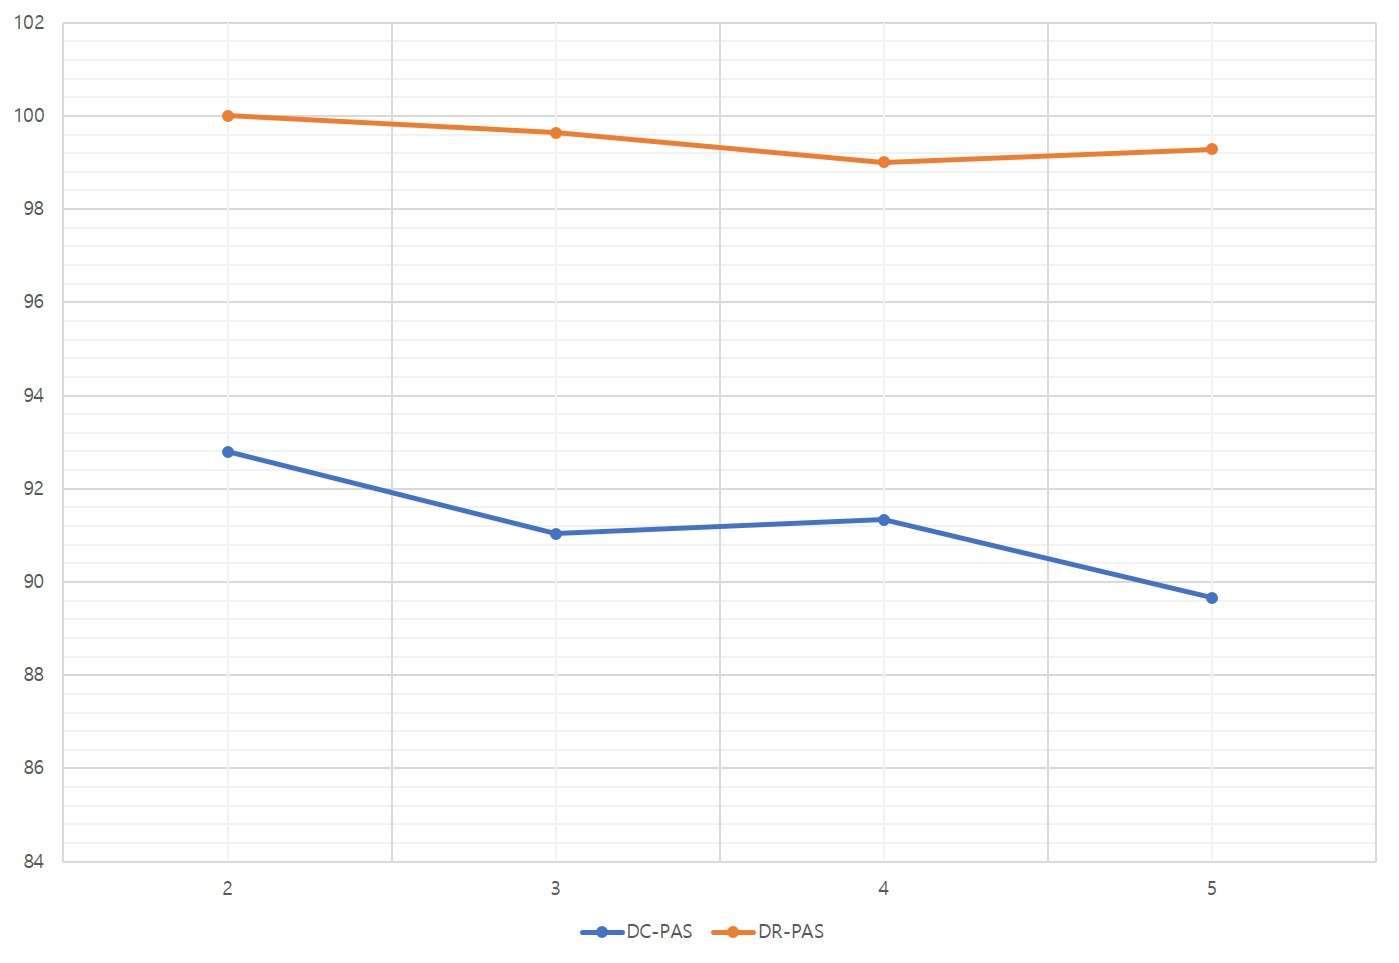
\includegraphics[width=3.6in, height=2.0in]{fig6.jpg}
\caption{Comparison on elapsed time of DR-TAS vs. DC-TAS}
\label{fig6}
}
\end{figure}


%%%%%%%%%%%%%%%%%%%%%%%%%%%%%%%%%%%%%%%%%%%%%%%%%%%%%%%%%%%%%%%%%%%%%%%%%%%%%%%%%%%%%%%%%%%%%%%%%%%%%%%%%%%%%%%%%%%%%%%%%%%%
% 5.conclusion
\section{Conclusion}
%%%%%%%%%%%%%%%%%%%%%%%%%%%%%%%%%%%%%%%%%%%%%%%%%%%%%%%%%%%%%%%%%%%%%%%%%%%%%%%%%%%%%%%%%%%%%%%%%%%%%%%%%%%%%%%%%%%%%%%%%%%%
As a result of learning from the LSTM model using network traffic data as a unit of flow, its accuracy was over 99$\%$. This confirmed that the classification was nearly 100$\%$.
Future research will explore the classification of network traffic through deployment in a real network and also how new packets, other than those already learned, will be classified as they enter the real network.

\ifCLASSOPTIONcaptionsoff
  \newpage
\fi


%%%%%%%%%%%%%%%%%%%%%%%%%%%%%%%%%%%%%%%%%%%%%%%%%%%%%%%%%%%%%%%%%%%%%%%%%%%%%%%%%%%%%%%%%%%%%%%%%%%%%%%%%%%%%%%%%%%%%%%%%%%%

\begin{thebibliography}{1}
\bibitem{Valentin2014}
Valentín Carela-Español, Tomasz Bujlow, and Pere Barlet-Ros: "Is Our Ground-Truth for Traffic Classification Reliable?",  {\it In Proc. of the Passive and Active Measurements Conference (PAM'14),} Los Angeles, CA, USA, March 2014.

\bibitem{Park2009}
Jinwan Park, ``statistics signiture based application traffic classification," {\it Korea Communication Journal,} vol. 34, pp. 1234--1244, Nov. 2009.

\bibitem{Risso2008}
F. Risso, ``Lightweight, Payload-Based Traffic Classification: An Experimental Evaluation," {\it IEEE International Conference on Communications 2008,}, 2008.

\bibitem{LeCun}
Yann LeCun, ``Deep Learning," {\it Nature International Weekly Journal of Science,}

\bibitem{Mikolov2011}
T. Mikolov, S. Kombrink, L. Burget, J. Cernocky and S. Khudanpur, ``Extensions of recurrent neural network language model," {\it 2011 IEEE International Conference on Acoustics, Speech and Signal Processing(ICASSP),} pp. 5528--5531, 2011.

\bibitem{Sak2014}
H. Sak, Andrew Senior and F. Beaufays, ``Long short-term memory recurrent neural network architectures for large scale acoustic modeling," {\it Proceedings of the Annual Conference of the International Speech Communication Association(INTERSPEECH),} pp. 338--342, Jan. 2014.





%%%%%%%%%%%%%%%%%%%%%%%%%%%%%%%%%%%%%%%%%%%%%%%%%%%%%%%%%%%%%%%%%%%%%%%%%%%%%%%%%%%%%%%%%%%%%%%%%%%%%%%%%%%%%%%%%%%%%%%%%%%%



\end{thebibliography}

\end{document}


 